\documentclass[twocolumn,english,notitlepage]{article}  
\usepackage[margin=2cm]{geometry}

% \setlength{\parindent}{0pt} % no indents

\usepackage{overhead} % Overhead is in a separate file

\title{Restricted and Unrestricted Coupled-Cluster Doubles Applied to Two-Dimensional Harmonically Oscillating Quantum Dots}
\author{Håkon Kvernmoen$^\dagger$ }

\date{\today}

\begin{document}


\twocolumn[
    \begin{@twocolumnfalse}
        \maketitle
        \begin{center}
            $^\dagger$ Implementation present at \url{https://github.com/hkve/coupled-cluster-FYS4411}
        \end{center}
        \begin{abstract}
                Implementation of Hartree-Fock (HF) and Coupled Cluster using doubles excitations (CCD) are benchmarked using a Quantum dot (QD), modeled as a two-dimensional Harmonic Oscillator (2DHO) potential. Application to $s$-type hydrogen states for Helium and Beryllium bypassed both HF and Configuration Interaction using single excitations (CIS). Implementations in both restricted and unrestricted schemes display a constant time improvement in favor of the restricted schemes, applicable to the closed shell systems used. Low frequency solutions were obtained for 2 and 6 particles giving $\omega_c < 0.01$ and $\omega_c = 0.0621$ respectively, where the electron-electron interaction strength is significantly higher than the confining HO potential. Comparisons with both variational and singles added schemes ($\Lambda-$CCSD, CCSD) present in the literature was performed, with deviations explained by the doubles' truncation presented in this work.
            \newline    
            \newline    
            \newline    
        \end{abstract}
    \end{@twocolumnfalse}
]

\tableofcontents

\section{Introduction}
\citep{hastie01statisticallearning}

\begin{align}
    F = ma \label[eq]{eq:test}
\end{align}

\cref{eq:test}

\section{Theory}
\subsection{Mathematical framework and notation}
In the following we will use the occupation representation, making use of creation $\crta{p}$ and annihilation $\ania{p}$ operators. As a shorthand, we will write $\crt{p} \equiv \crta{p}$ and $\ani{p} \equiv \ania{p}$ when no confusion can be made. $N$ represents the number of occupied states while $L$ the total number of states in our calculations. The indicies $p,q,\ldots$ are reserved for the $L$ general states, the $N$ occupied states are indexed by $i,j,\ldots$, while the $L-N$ unoccupied (virtual) states by $a,b,\ldots$ indicies.

Since we are treating fermionic systems, the canonical anticommutation relations are used

\begin{align*}
    \set{\crt{p},\crt{q}} = \set{\ani{p},\ani{q}} = 0 \hspace{20px} \set{\crt{p},\ani{q}} = \delta_{pq}.
\end{align*}
One and two body matrix elements are calculated using a computational basis, with explicit expressions for one body Hamiltonians $h(\vec{x})$ and two body interaction $v(\vec{x}, \vec{x}')$ here presented in position space

\begin{align*}
    \bra{p}\hat{h}\ket{q} &= \int \dd{\vec{x}} \psi_p^*(x) \hat{h}(\vec{x}) \psi_q(x) \\
    \elm{pq}{rs} &= \int \dd{\vec{x}}\dd{\vec{x}'} \psi_p^*(\vec{x})\psi_q^*(\vec{x}') \hat{v}(\vec{x},\vec{x}') \psi_r(\vec{x})\psi_s(\vec{x}')
\end{align*}
with $\psi_p$ being a single particle wave function, often chosen to be the eigenfunction of $\hat{h}$. Note that $p$ also contain the spin quantum number, meaning that $\dd \vec{x}$ implicitly contains a spin component. If $\hat{h}$ or $\hat{v}$ is spin \textit{independent}, this simply reduces to Kronecker deltas for the spin component. It is often convenient to use antisymmetrized matrix elements, defined as 
\begin{align*}
    \elmAS{pq}{rs} = \elm{pq}{rs} - \elm{pq}{sr}
\end{align*}
The shorthands $\hshort{p}{q} \equiv \bra{p} \hat{h} \ket{q}$, $\elmshort{pq}{rs} \equiv \elm{pq}{rs}$ and $\elmASshort{pq}{rs} \equiv \elmAS{pq}{rs}$ will often be used. Using this formulation, a general two-body operator can be constructed

\begin{align}
    \ham = \sum_{pq} \hshort{p}{q}\crt{p}\ani{q} + \frac{1}{4} \sum_{pqrs} \elmASshort{pq}{rs}\crt{p}\crt{q}\ani{s}\ani{r} \label[eq]{eq:theo:second_quant_ham}
\end{align}
The simplest ground state ansatz
\begin{align*}
    \ketansatz = \crt{i}\crt{j}\ldots \ket{0},
\end{align*}
can be evaluated to calculate the simplest energy guess
\begin{align}
    \braansatz \ham \ketansatz = \sum_{i} \hshort{i}{i} + \frac{1}{2}\sum_{ij} \elmASshort{ij}{ij} \equiv \Eref, \label[eq]{eq:theo:e0ref}
\end{align}
named the \textit{reference energy}. Commonly wicks theorem is applied to \cref{eq:theo:second_quant_ham} to pick out the \cref{eq:theo:e0ref} contribution, defining the \textit{normal ordered} Hamiltonian
\begin{align*}
    \ham &= \hamno + \Eref = \fockno + \interno + \Eref
\end{align*}
where $\fockno$ and $\interno$ is the normal ordered \textit{Fock operator} and two body interaction respectively.
\begin{align}
    \fockno &= \sum_{pq} \fshort{p}{q} \set{\crt{p} \ani{q}}, \\
    \interno &= \frac{1}{4}\sum_{pqrs} \elmASshort{pq}{rs} \set{\crt{p}\crt{q}\ani{s}\ani{r}}
\end{align}
The Fock operator matrix elements $\fshort{p}{q}$ are given as 
\begin{align*}
    \fshort{p}{q} = \hshort{p}{q} + \sum_i \elmASshort{pi}{qi}
\end{align*}
normal order, Hamiltonian, normal order Hamiltonian, 

\begin{align}
    \hat{H}\ket{\Psi} = E \ket{\Psi} \label[eq]{eq:theo:schroding_equation}
\end{align}

\subsection{Hartree-Fock}

\subsection{Coupled Cluster}
The exact solution $\ket{\Psi}$ is approximated by an exponential ansatz $\ketCC$ 
\begin{align}
    \ket{\Psi} \approx \ketCC \equiv \exp{\cluster{}} \ketansatz. \label[eq]{eq:theo:exponential_ansatz}
\end{align}
The operators $\cluster{} = \cluster{1} + \cluster{2} + \ldots$ acting on the ground state ansatz $\ketansatz$ are the so-called \textit{cluster operators} defined as
\begin{align}
    \cluster{m} = \frac{1}{(m!)^2} \sum_{\substack{ab\ldots\\ij\ldots}} \amplitude{ab\ldots}{ij\ldots} \set{\crt{a}\ani{i} \crt{b} \ani{j}\ldots} \label[eq]{eq:theo:cluster_operators_general}
\end{align}
where $m \leq N$. The scalars $\amplitude{ab\ldots}{ij\ldots}$ are unknown expansion coefficients called \textit{amplitudes}, which we need to solve for. All the creation and annihilation operators of \cref{eq:theo:cluster_operators_general} anticommute, giving the restriction that

\begin{align}
    \amplitude{\hat{P}(ab\ldots)}{\hat{P}'(ij\ldots)} = (-1)^{\sigma(\hat{P})+\sigma(\hat{P}')} \amplitude{ab\ldots}{ij\ldots}. \label[eq]{eq:theo:amplitude_permutation_symmetry}
\end{align}
Here $P$ and $P'$ permutes $\sigma(P)$ and $\sigma(P')$ indices respectively. This is the reason for the prefactor of \cref{eq:theo:cluster_operators_general}, since we have $m!$ ways to independently permute particle and hole indices. Instead of having $(L-N)^m N^m$ independent unknowns, we reduce this number by a factor of $(m!)^{2}$. 

\subsection{Doubles truncation}
Considering $N$ cluster operators in the exponential ansatz of \cref{eq:theo:exponential_ansatz} is not computationally feasible for realistic systems. The common practice is to include one or more $\cluster{m}$ operators, making a truncation on $\ketCC$ as well. In the following we will include only the double excitation operator $\cluster{2}$, know as the CCD approximation. This gives us 
\begin{align}
    \ket{\Psi} &\approx \ketCC \approx \ketCCD \equiv \exp{\cluster{2}} \ketansatz \label[eq]{eq:theo:CCD_exponential_ansatz}, \\
    \cluster{2} &= \frac{1}{4}\sum_{abij} \amplitude{ab}{ij}\set{ \crt{a} \ani{i} \crt{b}\ani{j}} \label[eq]{eq:theo:CCD_cluster},
\end{align}
with the four-fold amplitude permutation symmetry \footnote{For double amplitudes, the index permutation symmetry is equal to that of antisymmetrized two-body matrix elements $\elmAS{pq}{rs}$.},
\begin{align}
    \amplitude{ab}{ij} = - \amplitude{ba}{ij} = - \amplitude{ab}{ji} = \amplitude{ba}{ji}. \label[eq]{eq:theo:CCD_amplitude_symmetry}
\end{align}
Incorporating the CCD approximation in the Schr\"odinger equation (\cref{eq:theo:schroding_equation}), we see that
\begin{align}
    \ham \exp{\cluster{2}} \ketansatz &= E \exp{\cluster{2}} \nonumber \ketansatz,  \\
    \hamno \exp{\cluster{2}} \ketansatz &= \DECCD \exp{\cluster{2}} \ketansatz, \label[eq]{eq:theo:schroding_equation_CCD}
\end{align}
where $\DECCD = E-\Eref$. Expanding both sides and taking the inner product with $\braansatz$, we in principle get an equation for the energy. However, this approach is not amenable to practical computer implementation \citep{bartlettCoupledClusterMethodsMolecular1984} since the amplitude equation will be coupled with the energy equation. Therefor, we rather apply a similarity transform to \cref{eq:theo:schroding_equation_CCD} by multiplying by the inverse of $\exp{\cluster{2}}$,
\begin{align}
    \exp{-\cluster{2}} \hamno \exp{-\cluster{2}} \ketansatz &= \DECCD \ketansatz \nonumber \\
    \simham \ketansatz &= \DECCD \ketansatz \label[eq]{eq:theo:ccd_eigenvalueproblem}
\end{align}
where $\simham = \exp{-\cluster{2}} \hamno \exp{-\cluster{2}}$ is the similarity transformed Hamiltonian. Using this reformulated eigenvalue problem, we can perform the inner product with different states to calculate both $\DECCD$ and $\amplitude{ab}{ij}$. Considering $\braansatz$ we get

\begin{align}
    \braansatz \simham \ketansatz = \DECCD, \label[eq]{eq:theo:energy_equation_sim_transformed}
\end{align}
named the \textit{energy equation}. Considering excited states, we arrive at the \textit{amplitude equations}
\begin{align}
    \braexed{ab\ldots}{ij\ldots} \simham \ketansatz \label[eq]{eq:theo:amplitude_equations},
\end{align}
used for finding the unknown amplitudes $\amplitude{ab}{ij}$. To find explicit expressions for \cref{eq:theo:energy_equation_sim_transformed} and \cref{eq:theo:amplitude_equations}, we expand $\simham$ using the Hausdorff expansion
\begin{align*}
    \simham &= \hamno + \commutator{\hamno}{\cluster{2}} + \frac{1}{2!}\commutator{\commutator{\hamno}{\cluster{2}}}{\cluster{2}} + \ldots %&+ \frac{1}{4!}\commutator{\commutator{\commutator{\hamno}{\cluster{2}}}{\cluster{2}}}{\cluster{2}}
\end{align*}
fhjksd

\section{Method}
\subsection{Quantum Mechanical System}

\subsubsection{Helium and Beryllium}
The initial testing during development of the CCD and RCCD implementations was performed using Hydrogen wave functions. As a choice of basis sets, these functions are `physically motivated` in the sense of being solutions to the one body electron case. The well-know relevant quantum numbers determining the form of the spatial wave functions are $n$ as the principal quantum number, with $l$ and $m$ as orbital angular momentum and projection respectively. Due to the spherically symmetric potential, the wave function $\psi_{nlm}$ can be separated in a radial function $R_{nl}(r)$ and a spherical harmonic $\sphericalharmonic{m}{l}$,  

\begin{align}
    \psi_{nlm}(r,\theta,\phi) = R_{nl}(r) \sphericalharmonic{m}{l}(\theta, \phi). \label[eq]{eq:met:hydrogen_wf_definition}
\end{align}
The radial part $R_{nl}(r)$ has the form

\begin{align*}
    R_{nl}(r) &= A_{nl} e^{-r/na_0} \pclosed{\frac{2r}{na_0}}^l \bclosed{\associatedlaguerre{2l+1}{n-l-1}(2r/na_0)} \\
    A_{nl} &= \sqrt{ \pclosed{\frac{2}{na_0}}^3 \frac{(n-l-1)!}{2n(n+l)!} }
\end{align*}
With $L$ as the associated Laguerre polynomials and $a_0$ the Bohr radius. For $l > 0$ the Coulomb interaction integral of \cref{eq:met:hydrogen_wf_definition} can not be easily evaluated due to $\sphericalharmonic{m}{l}$ having a non-trivial $\theta$ and $\phi$ dependence. Therefor for simplicity we only consider $s$ orbital ($l=0$ states), when calculating $\elm{pq}{rs}$. This is briefly sketched in \cref{sec:app:hydrogen_coulomb_integrals}. The one-body term $\hshort{p}{q}$ are diagonal with 

\begin{align}
    h_{nm} = -\frac{Z}{2n^2}\delta_{nm}
\end{align}
We will be interested in calculating the ground state energy for Helium and Beryllium, with two and four electrons respectively. In addition to Hartree-Fock and CCD calculations, a comparison to configuration interaction using singles (CIS) will be performed for both Helium and Beryllium. The results will also be benchmarked against the famouse work done by Egil A. Hylleraas \citep{hylleraasNumerischeBerechnung2STerme1930}.

\subsubsection{Two-Dimensional Harmonic Oscillator}
\subsubsection{Doubly Magic Nuclei}
Define
\begin{align}
    R
\end{align}

\section{Results}
\subsection{Helium and Beryllium}
The closed shell Helium and Beryllium calculations are presented in \cref{tab:res:helium_and_beryllium}, with relative errors compared to FCI in \cref{tab:res:helium_and_beryllium_percent_error}. For both HF add CCD in both restricted and unrestricted schemes, no problems of convergence was encountered. Adding a mixing parameter $p > 0$ for CCD only resulted in slower convergence.

\begin{table}[H]
    \centering
    \begin{tabular}{cccccc}
    \toprule
        Atom      &  $\Eref$ & CI & FCI & HF & RHF\\
    \midrule
    He & -2.7500 & -2.8385 & -2.9037 & -2.8311 & -2.8311 \\
    Be & -13.7160 & -14.3621 & -14.6674 & -14.5083 & -14.5083 \\
    \bottomrule
    \end{tabular}
    \newline
    \vspace*{10px}
    \newline
    \begin{tabular}{ccccc}
        \toprule
        Atom & CCD & RCCD & CCD(HF) & RCCD(HF) \\
        \midrule
        He & -2.7516 & -2.7516 & -2.8391 & -2.8391 \\
        Be & -13.7195 & -13.7195 & -14.5129 & -14.5129 \\
        \bottomrule
    \end{tabular}
    \caption{Ground state energies for Helium and Beryllium in \au\hspace{2px}Calculations done with configuration interaction with both singles and no constraints (full), in addition to HF and CCD in both restricted and unrestricted schemes. }\label[tab]{tab:res:helium_and_beryllium}
\end{table}

\begin{table}[H]
    \centering
    \begin{tabular}{ccccc}
    \toprule
    Atom      &  $\Eref$ & CI  & HF & RHF\\
    \midrule
    He & 5.29 & 2.25  & 2.50 & 2.50 \\
    Be & 6.49 & 2.08  & 1.09 & 1.09 \\
    \bottomrule
    \end{tabular}
    \newline
    \vspace*{10px}
    \newline
    \begin{tabular}{ccccc}
        \toprule
        Atom & CCD & RCCD & CCD(HF) & RCCD(HF) \\
        \midrule
        He & 5.24 & 5.24 & 2.22 & 2.22 \\
        Be & 6.46 & 6.46 & 1.05 & 1.05 \\
        \bottomrule
    \end{tabular}
    \caption{ Relative error in \% for Helium and Beryllium from \cref{tab:res:helium_and_beryllium}, using the FCI results as the exact energies. }\label[tab]{tab:res:helium_and_beryllium_percent_error}
\end{table}

\subsection{Harmonic Oscillator}
Comparing with the analytical case of two interacting particles at $\omega = 1.0$ having an energy of $3.00$, the best results was achieved when using the 12 first shells as basis states. Here HF, CCD with HO basis and CCD with HF basis produced energies off (relative error) 3.161909 (5.397\%), 3.089302 (2.977\%) and 3.005879 (0.196\%) respectively. This gave a clear sign that the basis and algorithm implementations were set up correctly. The results from the restricted and unrestricted schemes were again identical.

A comparison of the elapsed time for each algorithm to converge is presented in \cref{fig:res:timing}. All runs were made using $N=2$. For $R > 9$, the unrestricted implementation begun slowing down substantially.  

\begin{figure}[H]
    \centering
    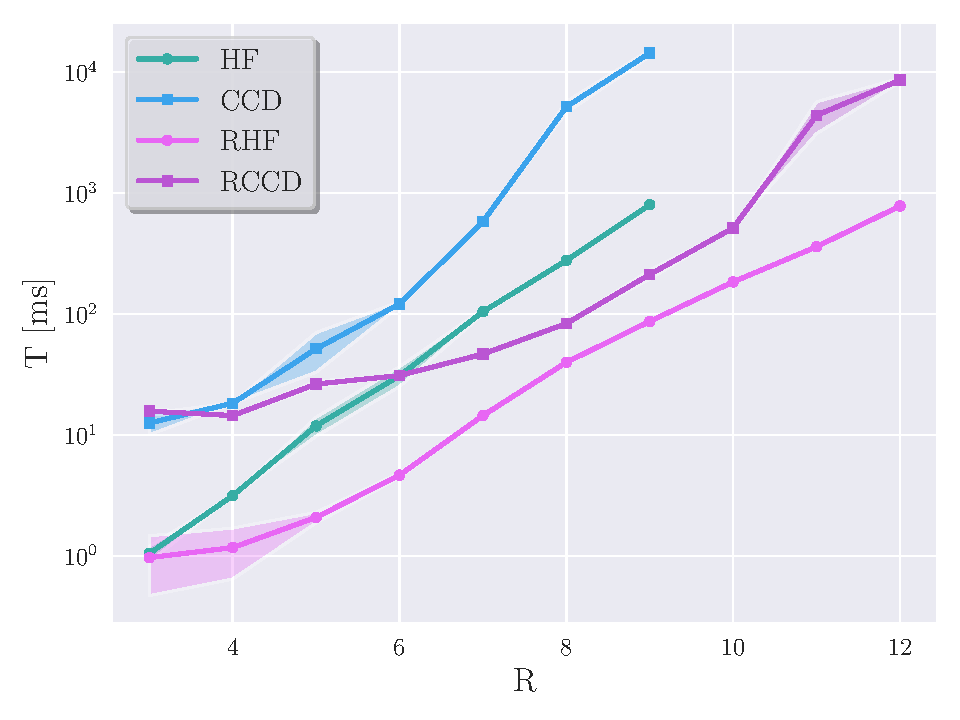
\includegraphics[width=\linewidth]{figs/timing.pdf}
    \caption{Showing elapsed time in milliseconds, comparing HF and CCD between the unrestricted and restricted schemes. $N=2$ particles were used, with time being averaged over ten runs. The shaded regions display the standard deviation over the ten runs.}\label[fig]{fig:res:timing}
\end{figure}
Due to the computational expense when using a large amount of virtual states, all other energy calculations were done in the restricted scheme.  Increasing the number of particles in the $\omega = 1.0$ system is presented in \cref{tab:res:ho_omega1}. For 12 and 20 particles, convergence for CCD using the HO basis was troublesome. This was in contrast to the HF basis, where no tuning of the mixing parameter was required. 

Lowering the frequency to $\omega = 0.5$, we show the same particle systems in \cref{tab:res:ho_omega0.5}. The convergence troubles still stood for the HO basis, but begun for smaller systems with a smaller number of virtual basis states. Here the 20 particle case also required tuning the mixing parameter for the HF basis, with $R > 7$ not achieving convergence with the parameters tested.
Lastly lowering the frequency all the way down to $\omega = 0.1$, the 2 and 6 particle systems are presented in \cref{tab:res:ho_omega0.1}. Using 12 and 20 particles did not result in any convergence and are therefor not shown.

Since convergence trouble with lower frequency and more particles was experienced, this was investigated further in \cref{fig:res:varying_omega}. Here the ground state energy over the non-interacting energy is drawn as a function of $\omega$. Here the realms of non-convergence is clearer, especially for $20$ particles.
\begin{figure}[H]
    \centering
    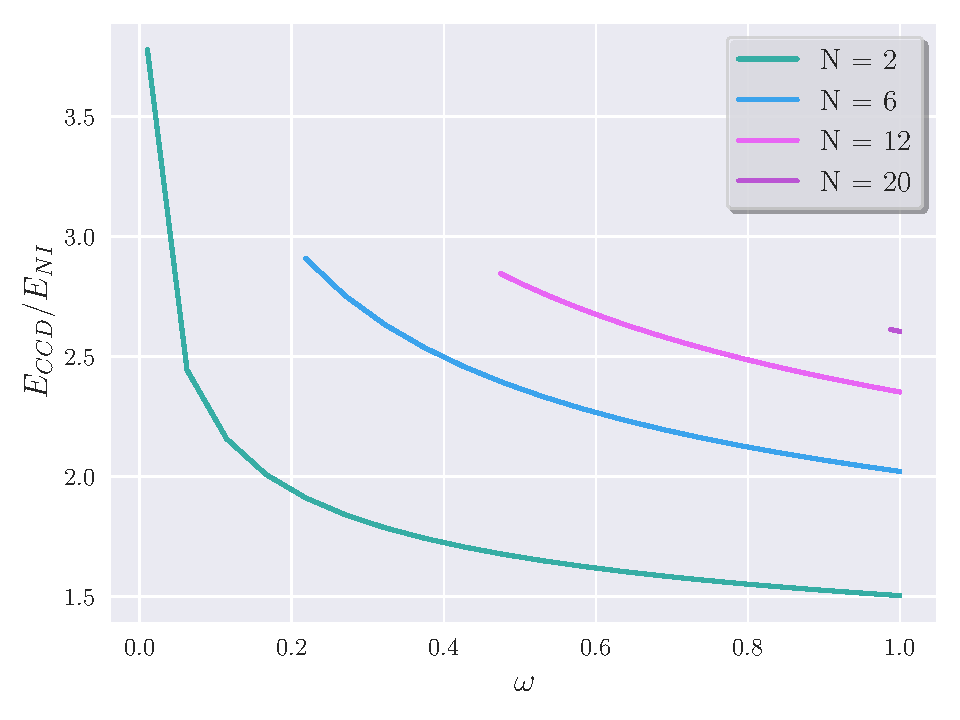
\includegraphics[width=\linewidth]{figs/vary_omega.pdf}
    \caption{Showing the ground state energy calculated using CCD ($E_{\text{CCD}}$) over the non-interacting solution ($E_{\text{NI}}$) as a function of $\omega$ for $N= 2, 6, 12$ and 20 particles. The lines stop when convergence could no longer be achieved.}\label[fig]{fig:res:varying_omega}
\end{figure}
\clearpage
% omega = 1.0 tables
\begin{table*}
    \begin{subtable}[h]{0.45\textwidth}
        \centering
        \begin{tabular}{cccc}
            \toprule
            $R$ & HF & CCD & CCD(HF) \\
            \midrule
            1 & 3.253314 & 3.253314 & 3.253314 \\
            2 & 3.253314 & 3.152329 & 3.152329 \\
            3 & 3.162691 & 3.141828 & 3.039049 \\
            4 & 3.162691 & 3.118684 & 3.025277 \\
            5 & 3.161921 & 3.110972 & 3.017946 \\
            6 & 3.161921 & 3.103343 & 3.013924 \\
            7 & 3.161909 & 3.099330 & 3.011408 \\
            8 & 3.161909 & 3.095925 & 3.009624 \\
            9 & 3.161909 & 3.093663 & 3.008351 \\
            10 & 3.161909 & 3.091818 & 3.007366 \\
            11 & 3.161909 & 3.090438 & 3.006599 \\
            12 & 3.161909 & 3.089302 & 3.005979 \\
            \bottomrule
        \end{tabular}
        \caption{$N = 2$}\label[tab]{tab:res:ho_omega1_N2}
    \end{subtable}
    \hfill
    \begin{subtable}[h]{0.45\textwidth}
        \centering
        \begin{tabular}{ccccc}
            \toprule
            $R$ & $p$ & HF & CCD & CCD(HF) \\
            \midrule
            2 & N & 22.219813 & 22.219813 & 22.219813 \\
            3 & N & 21.593198 & 21.974680 & 21.423816 \\
            4 & N & 20.766919 & 21.854198 & 20.429269 \\
            5 & N & 20.748402 & 21.793640 & 20.332466 \\
            6 & N & 20.720257 & 21.750086 & 20.274029 \\
            7 & N & 20.720132 & 21.718843 & 20.249851 \\
            8 & N & 20.719248 & 21.695225 & 20.234708 \\
            9 & 0.30 & 20.719248 & 21.675965 & 20.224387 \\
            10 & 0.30 & 20.719217 & 21.661863 & 20.217073 \\
            11 & 0.30 & 20.719215 & 21.649847 & 20.211538 \\
            12 & 0.30 & 20.719215 & 21.640798 & 20.207259 \\
            \bottomrule
        \end{tabular}
        \caption{$N = 6$}\label[tab]{tab:res:ho_omega1_N6}
    \end{subtable}
    \hfill
    \begin{subtable}[h]{0.45\textwidth}
        \centering
        \begin{tabular}{ccccc}
            \toprule
            $R$ & $p$ & HF & CCD & CCD(HF) \\
            \midrule
            3 & $>$0.99 & 73.765549 & 73.765549 & 73.765549 \\
            4 & $>$0.99 & 70.673849 & - & 70.324257 \\
            5 & $>$0.99 & 67.569930 & - & 67.031101 \\
            6 & $>$0.99 & 67.296869 & - & 66.526674 \\
            7 & $>$0.99 & 66.934745 & - & 66.049566 \\
            8 & $>$0.99 & 66.923094 & - & 65.972154 \\
            9 & $>$0.99 & 66.912244 & - & 65.921206 \\
            10 & $>$0.99 & 66.912035 & - & 65.889282 \\
            11 & $>$0.99 & 66.911365 & - & 65.866717 \\
            12 & $>$0.99 & 66.911364 & - & 65.849773 \\
        \bottomrule
    \end{tabular}
    \caption{$N = 12$}\label[tab]{tab:res:ho_omega1_N12}
\end{subtable}
    \hfill
    \begin{subtable}[h]{0.45\textwidth}
        \centering
        \begin{tabular}{ccccc}
            \toprule
            $R$ & $p$ & HF & CCD & CCD(HF) \\
            \midrule
            4 & $>$0.99 & 177.963297 & 177.963297 & 177.963297 \\
            5 & $>$0.99 & 168.808284 & - & 168.459454 \\
            6 & $>$0.99 & 161.339721 & - & 160.594508 \\
            7 & $>$0.99 & 159.958722 & - & 158.841116 \\
            8 & $>$0.99 & 158.400172 & - & 157.038328 \\
            9 & $>$0.99 & 208.177129 & - & 156.676039 \\
            10 & $>$0.99 & 158.017667 & - & 156.367932 \\
            11 & $>$0.99 & 158.010276 & - & 156.292420 \\
            12 & $>$0.99 & 158.004951 & - & 156.238255 \\
            \bottomrule
        \end{tabular}
        \caption{$N = 20$}\label[tab]{tab:res:ho_omega1_N20}
    \end{subtable}
    \caption{Showing ground state energies for $\omega = 1.0$, when increasing the number of shells $R$ used for the calculation up to and including $R=12$. The four entries \cref{tab:res:ho_omega1_N2},\cref{tab:res:ho_omega1_N6},\cref{tab:res:ho_omega1_N12} and \cref{tab:res:ho_omega1_N20} shows 2, 6, 12 and 20 particles respectively. Restricted schemes have been used for all calculations, with CCD and CCD(HF) using the HO and HF basis respectively. The column $p$ displays the mixing parameter for the HO basis used when convergence without it was not achieved, with `N` marking no mixing required. A dashed line `-` for the energy marks no convergence across different mixing parameters.}\label[tab]{tab:res:ho_omega1}
\end{table*}

% omega = 0.5 tables
\begin{table*}
    \begin{subtable}[h]{0.45\textwidth}
        \centering
        \begin{tabular}{cccc}
            \toprule
            $R$ & HF & CCD & CCD(HF) \\
            \midrule
            1 & 1.886227 & 1.886227 & 1.886227 \\
            2 & 1.886227 & 1.786915 & 1.786915 \\
            3 & 1.799856 & 1.778907 & 1.681981 \\
            4 & 1.799856 & 1.760121 & 1.673883 \\
            5 & 1.799748 & 1.754389 & 1.670056 \\
            6 & 1.799748 & 1.748238 & 1.667808 \\
            7 & 1.799745 & 1.745232 & 1.666479 \\
            8 & 1.799745 & 1.742551 & 1.665532 \\
            9 & 1.799743 & 1.740856 & 1.664848 \\
            10 & 1.799743 & 1.739446 & 1.664278 \\
            11 & 1.799742 & 1.738412 & 1.663866 \\
            12 & 1.799742 & 1.737563 & 1.663523 \\
            \bottomrule
        \end{tabular}
        \caption{$N = 2$}\label[tab]{tab:res:ho_omega0.5_N2}
    \end{subtable}
    \hfill
    \begin{subtable}[h]{0.45\textwidth}
        \centering
        \begin{tabular}{ccccc}
            \toprule
            $R$ & $p$ & HF & CCD & CCD(HF) \\
            \midrule
            2 & N & 13.640713 & 13.640713 & 13.640713 \\
            3 & N & 13.051620 & 13.385995 & 12.901525 \\
            4 & N & 12.357471 & 13.261110 & 12.057347 \\
            5 & $>$0.99 & 12.325128 & - & 11.935004 \\
            6 & $>$0.99 & 12.271499 & - & 11.864102 \\
            7 & $>$0.99 & 12.271375 & - & 11.849764 \\
            8 & $>$0.99 & 12.271361 & - & 11.841326 \\
            9 & $>$0.99 & 12.271337 & - & 11.835472 \\
            10 & $>$0.99 & 12.271326 & - & 11.831348 \\
            11 & $>$0.99 & 12.271324 & - & 11.828237 \\
            12 & $>$0.99 & 12.271320 & - & 11.825837 \\
            \bottomrule
        \end{tabular}
        \caption{$N = 6$}\label[tab]{tab:res:ho_omega0.5_N6}
    \end{subtable}
    \hfill
    \begin{subtable}[h]{0.45\textwidth}
        \centering
        \begin{tabular}{ccccc}
            \toprule
            $R$ & $p$ & HF & CCD & CCD(HF) \\
            \midrule
            3 & $>$0.99 & 46.361130 & 46.361130 & 46.361130 \\
            4 & $>$0.99 & 43.663267 & - & 43.309862 \\
            5 & $>$0.99 & 41.108851 & - & 40.654710 \\
            6 & $>$0.99 & 40.750512 & - & 40.068342 \\
            7 & $>$0.99 & 40.302719 & - & 39.508497 \\
            8 & $>$0.99 & 40.263752 & - & 39.399125 \\
            9 & $>$0.99 & 40.216688 & - & 39.329313 \\
            10 & $>$0.99 & 40.216252 & - & 39.309411 \\
            11 & $>$0.99 & 40.216195 & - & 39.296003 \\
            12 & $>$0.99 & 40.216165 & - & 39.285970 \\
            \bottomrule
        \end{tabular}
        \caption{$N = 12$}\label[tab]{tab:res:ho_omega0.5_N12}
    \end{subtable}
    \hfill
    \begin{subtable}[h]{0.5\textwidth}
        \centering
        \begin{tabular}{cccccc}
            \toprule
            $R$ & $p$ & $p(HF)$ & HF & CCD & CCD(HF) \\
            \midrule
            4 & $>$0.99 & N & 113.412648 & 113.412648 & 113.412648 \\
            5 & $>$0.99 & 0.20 & 105.227282 & - & 104.896465 \\
            6 & $>$0.99 & 0.20 & 99.754600 & - & 99.119518 \\
            7 & $>$0.99 & $>$0.99 & 131.446882 & - & - \\
            8 & $>$0.99 & $>$0.99 & 133.900840 & - & - \\
            9 & $>$0.99 & $>$0.99 & 134.132319 & - & - \\
            10 & $>$0.99 & $>$0.99 & 133.574242 & - & - \\
            11 & $>$0.99 & $>$0.99 & 133.244135 & - & - \\
            12 & $>$0.99 & $>$0.99 & 133.178089 & - & - \\
            \bottomrule
        \end{tabular}
        \caption{$N = 20$}\label[tab]{tab:res:ho_omega0.5_N20}
    \end{subtable}
    \caption{Showing ground state energies for $\omega = 0.5$, when increasing the number of shells $R$ used for the calculation up to and including $R=12$. The four entries \cref{tab:res:ho_omega0.5_N2},\cref{tab:res:ho_omega0.5_N6},\cref{tab:res:ho_omega0.5_N12} and \cref{tab:res:ho_omega0.5_N20} shows 2, 6, 12 and 20 particles respectively. Restricted schemes have been used for all calculations, with CCD and CCD(HF) using the HO and HF basis respectively. The columns $p$ and $p(HO)$ displays the mixing parameter used for the HO and HF basis respectively when convergence without it was not achieved, with `N` marking no mixing required. A dashed line `-` for the energy marks no convergence across different mixing parameters.}\label[tab]{tab:res:ho_omega0.5}
\end{table*}

\begin{table*}    
    \begin{subtable}[h]{0.45\textwidth}
        \centering
        \begin{tabular}{cccccc}
            \toprule
            $R$ & $p$ & $p(HF)$ & HF & CCD & CCD(HF) \\
            \midrule
            1 & N & N & 0.596333 & 0.596333 & 0.596333 \\
            2 & N & N & 0.596333 & 0.512521 & 0.512521 \\
            3 & N & N & 0.526903 & 0.505981 & 0.442244 \\
            4 & N & N & 0.526903 & 0.499233 & 0.442018 \\
            5 & 0.30 & N & 0.525666 & 0.497206 & 0.443337 \\
            6 & 0.30 & N & 0.525666 & 0.494263 & 0.443147 \\
            7 & 0.30 & N & 0.525635 & 0.493172 & 0.443050 \\
            8 & 0.30 & N & 0.525635 & 0.498285 & 0.442974 \\
            9 & 0.30 & N & 0.525635 & 0.491290 & 0.442921 \\
            10 & 0.30 & N & 0.525635 & 0.490676 & 0.442887 \\
            11 & 0.50 & N & 0.525635 & 0.490305 & 0.442856 \\
            12 & 0.50 & 0.30 & 0.525635 & 0.489960 & 0.442849 \\
            \bottomrule
        \end{tabular}
        \caption{$N = 2$}\label[tab]{tab:res:ho_omega0.1_N2}
    \end{subtable}
    \hfill
    \begin{subtable}[h]{0.45\textwidth}
        \centering
        \begin{tabular}{cccccc}
            \toprule
            $R$ & $p$ & $p(HF)$ & HF & CCD & CCD(HF) \\
            \midrule
            2 & $>$0.99 & N & 4.864244 & 4.864244 & 4.864244 \\
            3 & $>$0.99 & N & 4.435740 & - & 4.319916 \\
            4 & $>$0.99 & N & 4.019787 & - & 3.829968 \\
            5 & $>$0.99 & N & 3.963148 & - & 3.666723 \\
            6 & $>$0.99 & N & 3.870617 & - & 3.597876 \\
            7 & $>$0.99 & 0.30 & 3.863135 & - & 3.590411 \\
            8 & $>$0.99 & 0.30 & 3.852880 & - & 3.587734 \\
            9 & $>$0.99 & 0.30 & 3.852591 & - & 3.587314 \\
            10 & $>$0.99 & 0.30 & 3.852393 & - & 3.587159 \\
            11 & $>$0.99 & 0.30 & 3.852391 & - & 3.586844 \\
            12 & $>$0.99 & 0.30 & 3.852382 & - & 3.586606 \\
            \bottomrule
        \end{tabular}
        \caption{$N = 6$}\label[tab]{tab:res:ho_omega0.1_N6}
    \end{subtable}
    \caption{Showing ground state energies for $\omega = 0.1$, when increasing the number of shells $R$ used for the calculation up to and including $R=12$. The four entries \cref{tab:res:ho_omega0.1_N2} and \cref{tab:res:ho_omega0.1_N6} shows 2 and 6 particles respectively. Restricted schemes have been used for all calculations, with CCD and CCD(HF) using the HO and HF basis respectively. The columns $p$ and $p(HO)$ displays the mixing parameter used for the HO and HF basis respectively when convergence without it was not achieved, with `N` marking no mixing required. A dashed line `-` for the energy marks no convergence across different mixing parameters.}\label[tab]{tab:res:ho_omega0.1}
\end{table*}
\clearpage

\section{Discussion}
\subsection{Helium and Beryllium}
The Helium and Beryllium calculations were presented in \cref{tab:res:helium_and_beryllium}. Comparing with the FCI calculated the values, we see from the relative error \cref{tab:res:helium_and_beryllium_percent_error} that performing a CCD calculation using either the Hydrogen basis or HF basis improved over the reference energy in each scheme. Comparing CI with HF, we see that CI performed better for Helium while HF actually performing substantially better for Beryllium. CCD using the HF basis did beat both CI and HF in both cases, however the margins were not enormous.

The Hylleraas result \citep{hylleraasNumerischeBerechnung2STerme1930} was $-79.005 \text{ eV}$ or $-2.903$ in atomic units is however much more precise. Inclusion of larger parts of the space, such as considering CISD as CCSD would improve results. Small basis sets such as this could serve as a good benchmarking system going forwards with the more complex solvers.

One could of course also expand the space, including more and more $s$-orbitals. There is however a quite limiting basis when only $l=0$ basis states are included. Lifting the $l = 0$ was explored in this work, however difficulties trough  angular integrands arose, such as

\begin{align*}
    \frac{|\sphericalharmonic{m_1}{l_1}(\theta_1,\phi_1)|^2|\sphericalharmonic{m_2}{l_2}(\theta_2,\phi_2)|^2}{\sqrt{r_1^2 + r_2 ^2 - 2r_1 r_2 \cos \theta_2 }}.
\end{align*}
Further investigation into integration techniques concerning spherical harmonics would be required. The algebraic solver \verb|SymPy| did require a lot of `hand holding` in terms of the $s$-integrals, and presumably this would also be the case when considering less trivial angular integrals. Using one of the many Slater-type orbitals (STOs) or Gaussian-type orbitals (GTOs) is commonly the preferred method in the literature, having closed form recursion relation and being well documented. The problem of $l \neq 0$ integrals might be one of the reasons why Hydrogen-like orbitals are not as prevalent, despite being physically motivated for smaller atoms.  

\subsection{Performance}
Considering the time benchmarking from \cref{fig:res:timing}, it was clear that the restricted implementations were a worthwhile task. For $R > 9$, the unrestricted CCD had a quite large gap in performance. This could be due to the $\mathcal{O}(M^4 N^2)$ scaling from \cref{eq:met:term_to_be_optimized}, however another hypothesis is the memory usage. In the naive storage scheme where $\elmASshort{pq}{rs}$ needs to store $L^4$ elements, $R = 10$ would 

Better storage schemes such as matrix representations mapping $ij \rightarrow I$ and $ab \rightarrow A$ could increase computational performance, due to better usage of \verb|BLAS| functionality. This was not done however due to the main performance focus being comparing restricted to unrestricted schemes. In future work, a more systemic consideration of computational complexity would be desirable, pushing the limits on larger basis sets.



\subsection{Harmonic Oscillator}
Comparing with the analytical result for $\omega = 1.0$ and two particles, the relative error using a HO and HF basis have 2.997\% and 0.196\% respectively with $R=12$ basis states. This difference is quite more substantial compared with the Helium and Beryllium results. This indicates that the mean field approximation of the average electron-electron interaction is somewhat representative of the system. On the other hand, a simple HF calculation produced a relative error of 5.397\%, meaning that electron-electron correlations also play an important role when one wishes to describe the system more accurately. Comparing with \citep{pedersenlohneInitioComputationEnergies2011}, the same potential using $R=12$ shells as basis states yielded a relative error of $0.0218\%$. This indicates that the inclusion of singles excitations also plays an important role to achieve high precision results.
\subsubsection{Increasing the Number of Particles}
From the detailed $\omega = 1.0$ for 2, 6, 12 and 20 particles \cref{tab:res:ho_omega1} the energy per particle increases. For $N=2$ we have $E/N = 1.502990$, increasing to 3.367877 for $N=6$ and 5.487481 for $N=12$, while the $N = 20$ case tops it off with $E/N=7.811913$. Comparing with the non-interacting solutions of 1.00, 1.67, 2.34 and 3.00, we move from having $\sim 150\%$ of the non-interacting solution for 2 particles to $\sim 260\%$ for 20 particles. It is clear that adding more interactive particles in the trap increases the energy due to electron-electron repulsion.

Convergence using the HO basis was difficult for 12 and 20 particles. This can be explained by the true eigenstates of the interacting system deviating from the HO solution when the interaction plays a larger role. By making linear combinations of HO basis states and accounting for some electron-electron interaction by a mean field approximation, more accurate single particle eigenstates are created and thus convergence was achieved using the HF basis.

\subsubsection{Turing the Frequency Down}
The $\omega = 0.5$ results from \cref{tab:res:ho_omega0.5} yielded an energy per particle of 0.831762, 1.970973 and 3.273831 for 2, 6 and 12 particles respectively. Comparing with the non-interacting case for 0.5, we contain $\sim 160\%,\sim 240\%$ and $\sim 280\%$ of the non-interacting solution for 2, 6 and 12 particles. Thus decreasing the frequency makes the electron-electron repulsion play a bigger role than the HO trap. Making the HF basis converge is an easier job than the HO basis for the same reasons as for the $\omega = 1.0$ case, just more prevalent due to the interaction playing a bigger role. Additionally, achieving convergence for 20 particles using the HF basis also presented some problems. There are two reasons for this.

Firstly CC is perturbative in nature, meaning that when the non-interacting single particle energies moves closer and closer (since the frequency decreases), we move towards an almost degenerate state. As seen in \cref{eq:met:amplitudes_update_rule}, we divide by the diagonal Fock matrix, where the main contribution is the single particle energies. When  $\epsilon_a + \epsilon_b - \epsilon_i - \epsilon_j \rightarrow 0$, the new amplitude contribution will be inflated. This can be counteracted by turning up the mixing parameter $p$, but this might yield slow or no convergence of the amplitudes.

Secondly for low frequencies, the electron-electron repulsion be so large that the HO trap is not strong enough to contain the particles, such that we actually have an unbound system. For an unbound system, the HO solutions are not the correct basis states despite showing much of the same sinusoidal behavior as the free particle.   

These effects are even more prevalent for the $\omega = 0.1$ system \cref{tab:res:ho_omega0.1}, where convergence was only possible for 2 and 6 particles. Here the system is suspected to be unbound when filling the $R=3$ shell completely.

Defiantly mention
\begin{enumerate}
    \item CC not variational bad.
    \item HF basis good
    \item \st{Hydrogen $l \neq 0$ difficult.}
    \item \st{Lower frequencies harder for convergence.}
    \item \st{Not having singles when comparing to article}
    \item How much does energy improve from ref to HF compared to HF to CCD
\end{enumerate} 




\section{Concluding remarks} 
The implementations of HF and CCD, in both restricted and unrestricted schemes were successful. Benchmarking the $s$-orbital hydrogen basis, we found that CCD using a HF basis outperformed CIS for both Helium and Beryllium. The improvement over CI was particularly good for Beryllium, reducing the relative error from $2.08\%$ for CI to $1.05\%$ for CCD using a HF basis. However, most of the improvement was achieved due to the HF basis being particularly good.

For the QD, the $N = 2, \omega = 1.0$ analytical result was reproduced using $12$ shells with a relative error of only $0.196\%$. Here HF produced a relative error of $5.397\%$, which displays that electron correlations is an important factor in the HO system. Increasing the number of particles increased the energy per particle, as expected by the non-extensivity of the electron-electron repulsion. Decreasing the frequency  entailed convergence problems, which was identified as problems with the computational basis since the interaction became more prevalent than the HO potential. For 2 and 6 particles, low frequency solutions were obtained giving critical frequencies of $<0.010$ and $0.0061$ respectively.

The extra considerations with explicitly summing spin out of the equations was expedient, as was found when benchmarking runtime between the different methods. Further work would be to optimize even more, making use of intermediates for the RCCD implementation and matrix storage of elements and amplitudes.
\clearpage

% \printbibliography
\newpage
\bibliography{refs/references}
% for numbering appendix equations more appropriately
\numberwithin{equation}{section}
\renewcommand{\theequation}{\thesection.\arabic{equation}}
\newpage

\section{Appendix}
\begin{appendices}
    \section{Hydrogen Coulomb integrals}\label[sec]{sec:app:hydrogen_coulomb_integrals}
Considering states without orbital angular momentum, we remove the dependence on the two quantum numbers $l$ and $m$, giving

\begin{align*}
    &\psi_{nlm}(r,\theta,\phi) \longrightarrow \psi_n (r,\theta, \phi) \\
    &= \sqrt{\pclosed{\frac{4}{n^5}} } e^{-r/n} \associatedlaguerre{1}{n-1}(2r/n) \sphericalharmonic{0}{0}.
\end{align*}
Where we work in distances of the Bohr radius $r/a_0 \longrightarrow r$. Since the Coulomb integral is over two $\vec{r}_1, \vec{r}_2 \in \mathbb{R}^3$ spaces, we align $\vec{r}_1$ along the $y$-axis and perform the $\vec{r}_2$ integral first. In spherical coordinates, the Coulomb interaction then becomes 

\begin{align}
    \hat{v}(\vec{r}_1, \vec{r}_2) = \frac{Z}{|\vec{r}_1 - \vec{r}_2|} = \frac{Z}{\sqrt{r_1^2 + r_2 ^2 - 2r_1 r_2 \cos \theta_2 }} \label[eq]{eq:app:coulomb_interaction}
\end{align}
With these preparations, the integrals can be solved for all $p,q,r,s$ combinations. The integrals were solved using \verb|SymPy| \citep{10.7717/peerj-cs.103} 
\end{appendices}


\end{document}

